\documentclass[11pt, a4paper]{article}
\usepackage{amsfonts}
\usepackage{geometry}
\usepackage{graphicx}
\usepackage{caption}
\usepackage{subcaption}
\usepackage{mathtools}
\usepackage{fontspec}
\geometry{a4paper, total={170mm,257mm}, left=20mm, top=20mm,}
\usepackage{hyperref}
\hypersetup{
    colorlinks,
    citecolor=green,
    filecolor=black,
    linkcolor=red,
    urlcolor=black
}
\usepackage{pgfplots}
\pgfplotsset{compat=1.18}
\pgfplotsset{width=10cm,compat=1.9}
\usepackage{tikz}
\usepackage{tikz-cd}
\usetikzlibrary{cd}
\usepackage{pgfmath}
\usepackage{amsmath}

\newcommand{\Proj}{\mathbb{P}}
\newcommand{\Aff}{\mathbb{A}}
\newcommand{\N}{\mathbb{N}}
\newcommand{\R}{\mathbb{R}}
\newcommand{\Z}{\mathbb{Z}}
\newcommand{\C}{\mathbb{C}}
\newcommand{\V}{\mathbb{V}}
\newcommand{\Lr}{\mathcal{O}}
\newcommand{\m}{\mathfrak{m}}
\newcommand{\ufd}{\textbf{UFD}}
\newcommand{\ann}{\mathfrak{a}\mathfrak{n}\mathfrak{n}}

\newtheorem{theorem}{Theorem}
\newtheorem{proposition}{Proposition}
\newtheorem{definition}{Definition}

\title{Commutative Algebra for Algebraic Geometry}
\author{Bailey Arm}

\begin{document}
\maketitle
\tableofcontents

\part{Algebraic Geometry, Hartshorne}
In this part, I will be going through the work of Hartshorne as he laid out in \cite{hartshorne2013algebraic}. The book is sectioned into 5 distinct chapters - 'Varieties', 'Schemes', 'Cohomology', 'Curves' and 'Surfaces'. We study them in order as they flow nicely. 

\section{Varieties}

\begin{definition}
\textbf{Affine $n$-Space over $k$: } Let $k$ be a field and $n \in \N$. Then the affine $n$-space over $k$ is defined
\[\Aff_k^n = \{(k_1,...,k_n)\in k^n\}\]
\end{definition}
It seems that this is a silly definition, but later on we will see that it is useful to have a distinction between the variety $\Aff^n_k$ and the set of points in $k^n$. We later view $\Aff_k^n$ as an affine variety - an object in some arbitrary space rather than the set of $k$-tuples. 

Let $A = k[x_1,...,x_n]$ be the polynomial ring over $k$ in $n$ variables. Then $f\in A$ is a map $f: k^n \to k$. We define the vanishing locus of this function in the following way:

\begin{definition}
    \textbf{Vanishing Locus of a Polynomial: }Let $f\in A = k[x_1,...,x_n]$, then the vanishing locus is
    \[\V(f) := \{p\in \Aff_k^n: f(p) = 0\}\]
\end{definition}

We can develop a more advanced analogue of this:
\begin{definition}
    \textbf{Vanishing Locus of a Set of Polynomials: }Let $T = \{f_i\}_{i \in I} \subset A = k[x_1,...,x_n]$, then the vanishing locus of $T$ is
    \[\V(T) := \{p\in \Aff_k^n: f(p) = 0, \quad \forall f \in T\}\]
\end{definition}

Some examples:

\begin{figure}[h]
    \centering
    \begin{subfigure}[b]{0.45\textwidth}
        \centering
        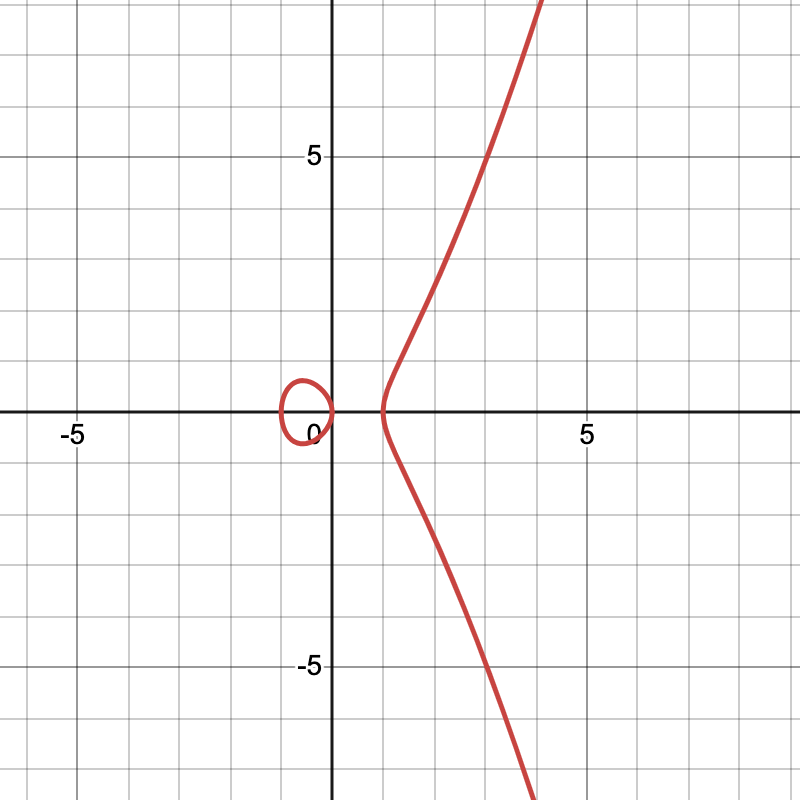
\includegraphics[scale = 0.2]{images/Varieties/desmos-graph2.png}
        \caption{$\V(y^2 - x(x+1)(x-1))$}
    \end{subfigure}
    \hfill
    \begin{subfigure}[b]{0.45\textwidth}
            \centering
            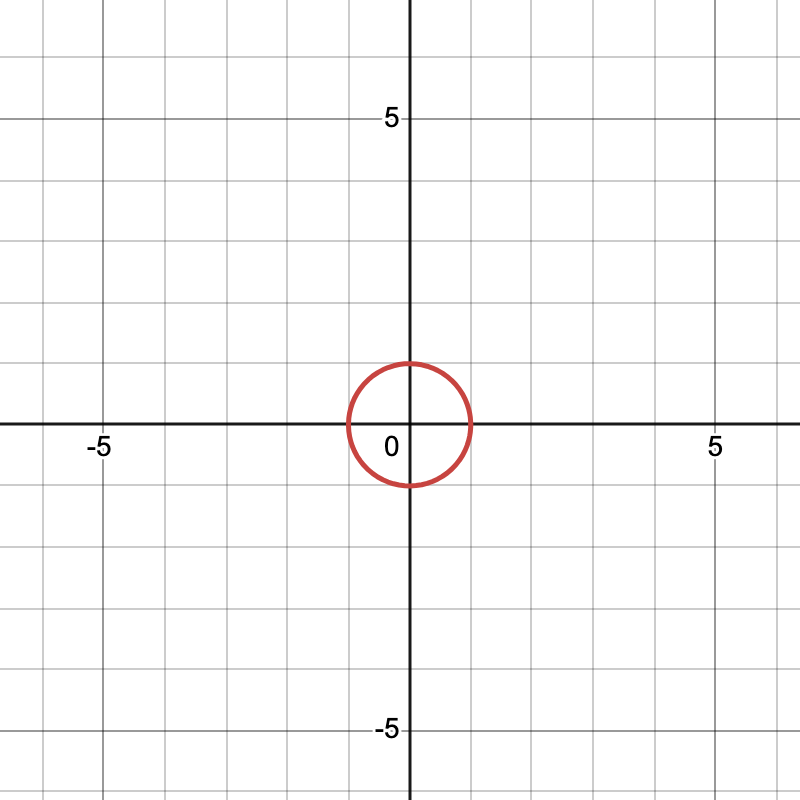
\includegraphics[scale = 0.2]{images/Varieties/desmos-graph.png}
            \caption{$\V(x^2 + y^2 - 1)$}
    \end{subfigure}
\caption{The vanishing locus of two separate polynomials plotted in $\R^2$}
\end{figure}

\subsection{Affine Varieties}
\subsection{Projective Varieties}
\subsection{Morphisms}
\subsection{Rational Maps}
\subsection{Nonsingular Varieties}
\subsection{Nonsingular Curves}
\subsection{Intersections in Projective Space}

\section{Schemes}
\subsection{Sheaves}
\subsection{Schemes}
\subsection{First Properties of Schemes}
\subsection{Separated and Proper Morphisms}
\subsection{Sheaves of Modules}
\subsection{Divisors}
\subsection{Projective Morphisms}
\subsection{Differentials}
\subsection{Formal Schemes}

\section{Cohomology}
\subsection{Derived Functors}
\subsection{Cohomology of Sheaves}
\subsection{Cohomology of a Noetherian Affine Scheme}
\subsection{Cech Cohomology}
\subsection{The Cohomology of Projective Space}
\subsection{Ext Groups and Sheaves}
\subsection{The Serre Duality Theorem}
\subsection{Higher Direct Images of Sheaves}
\subsection{Flat Morphisms}
\subsection{Smooth Morphisms}
\subsection{The Theorem on Formal Functions}
\subsection{The Semicontinuity Theorem}

\section{Curves}
\subsection{Riemann-Roch Theorem}
\subsection{Hurwitz's Theorem}
\subsection{Embeddings in Projective Space}
\subsection{Elliptic Curves}
\subsection{The Canonical Embedding}
\subsection{Classification of Curves in $\Proj^3$}

\section{Surfaces}
\subsection{Geometry on a Surface}
\subsection{Ruled Surfaces}
\subsection{Monoidal Transformations}
\subsection{The Cubic Surface in $\Proj^n$}\
\subsection{Birational Transformations}
\subsection{Classification of Surfaces}
\part{Commutative Geometry with a View Toward Algebraic Geometry, Eisenbud}

\section{Preliminaries}
\subsection{Rings and Ideals}
\begin{definition}
    \textbf{Ring}: A ring is an abelian group $R$ with a multiplication operation $*: R\times R\to R$ as well as an identity element $1\in R$ such that:
    \[a(bc) = (ab)c \quad \forall a,b,c\in R\]
    \[a(b + c) = ab + ac \quad \forall a,b,c \in R\]
    \[(b + c)  = ba + ca \quad \forall a,b,c\in R\]
    \[1a = a1 = a \quad \forall a\in R\]
\end{definition}
A ring is commutative if the ring commutes with respect to multiplication, that is $ab = ba \quad \forall a,b\in R$.

\begin{definition}
    \textbf{A Unit in a Ring: }Let $R$ be a ring. An element $u\in R$ is a unit if it is invertible, that is there exists some $v\in R$ such that $vu = 1 \in R$. 
\end{definition}

\begin{proposition}
    \textbf{Uniqueness of the Multiplicative Inverse of an Element in a Ring: }Let $u\in R$ where $R$ is a ring. Then $us = ut = 1\implies s = t$, i.e. inverses are unique in $R$ and we can speak of 'the' inverse of $u$.
\end{proposition}

\textit{Proof} Consider the same set up. Then we have $su = 1 = ut$ \footnote{It seems that we have used commutativity of $R$ here but we have not. If $us = 1$ then $(su)s = s(us) = s \implies su = (su)s s^{-1} = s s^{-1} = 1$}. We then have
\begin{equation*}
\begin{split}
    s &= s1 \\
    &= s (ut) \\
    &= (su) t \\
    &= t
\end{split}
\end{equation*}
So we are done.

\begin{definition}
    \textbf{Field: }A field is a non-zero ring such that every non-zero element is invertible. 
\end{definition}

\begin{definition}
    \textbf{Zero Divisor of a Ring: }Let $R$ be a ring. A zero-divisor in $R$ is a non-zero element $u$ such that there is another non-zero element $s$ with $us = 0$
\end{definition}

Whilst this seems rather abstract, zero divisors crop up more frequently than you would imagine. For example if we consider the hours on a clock, with the multiplication operation between hours being the usual one (that is the hour 3 multiplied by the hour 5 is the hour 15, but on a clock this would be the hour 3), then we have zero-divisors for any integer $n$ such that there is some $k$ with $nk = 12m$ for some $m\in \{0,...,11\}$. For example $3,4$ are a pair of zero-divisors, $2,6$ is another example.

\begin{definition}
    \textbf{Ideal of a Ring: }Let $R$ be a ring. An ideal $I$ in $R$ is an additive subgroup such that if $r in R, s\in I$ then $rs \in I$. An ideal $I$ is said to be generated by the subset $\mathcal{S} \subseteq I$ if any element in $I$ can be expressed as a linear combination (over $R$) of elements in $S$. More specifically,
    \[\exists \theta_1,...,\theta_n \in R, s_1,...,s_n \in \mathcal{S}: r = \sum_{i = 1}^n \theta_i s_i\]
\end{definition}

Some important notes here. A ring is \textbf{principal} if it is generated by a single element, in which case we write $I = (s)$. An ideal $I \subset R$ is prime if for any $f,g \in R$, if we have $fg\in I$ then either $f$ or $g$ is in $I$. A ring $R$ is a domain if $(0)$ is a prime ideal.\footnote{This seems like a weird definition at first, but it is equivalent to not having any zero-divisors. If $fg\in (0)$ then $(0)$ prime would men either $f= 0$ or $g = 0$, i.e. no zero-divisors} A maximal ideal of $R$ is a proper ideal $\mathfrak{m}$ that is not contained in any other ideal. Moreover, if $\mathfrak{m}$ is a maximal ideal, then $R/\mathfrak{m}$ is a field. 

\begin{proposition}
    Let $R$ be a ring and $\m$ a maximal ideal of $R$. Then $R/\m$ is a field. 
\end{proposition}

\begin{definition}
    \textbf{Commutative Algebra over a Ring: }Let $R$ be an abelian ring. A commutative algebra over $R$ is a commutative ring $S$ with a ring homomorphism $\alpha: R\to S$.
\end{definition}

\begin{proposition}
    Any ring is an algebra over the ring over integers $\Z$. 
\end{proposition}

\begin{definition}
    \textbf{Subalgebras: }Let $S$ be an algebra over a commutative ring $R$. A subring $S'$ is a commutative $R$-subalgebra of $S$ if $\text{Im}(\alpha) = \alpha(R) \subset S'$
\end{definition}

A homomorphism of $R$-algebras $\phi : S\to T$ is a homomorphism of rings such that $\phi(rs) = r\phi(s) \quad \forall r\in R, s\in S$. 

\subsubsection{Unique Factorisation}
Let $R$ be a ring. An element $r\in R$ is irreducible if it is not a unit and $r = st$ implies that one of $s,t$ is a unit in $R$. A ring $R$ is a \ufd  if any factorisation is unique up to scaling by units in $R$. 

\subsubsection{Modules}
\begin{definition}
    \textbf{Modules over Rings: }Let $R$ be a ring. An $R$-module $M$ is an abelian group together with an action with $R$, i.e. a map $\R\times M\to M$ expressed as $(r,m)\to rm$ satisfying $\forall r,s\in R, mn\in M$:
    \begin{itemize}
        \item $r(sm) = (rs)m$ 
        \item $r(m + n) = rm + rn$ 
        \item $(r + s)m = rm + sm$
        \item $1m = m$
    \end{itemize}
\end{definition}
The most interesting $R$-modules are those that take the form of ideals $I$ and their corresponding factor rings $R/I$. If $M$ is an $R$-module then the annihilator of $M$ is 
\[\ann_R(M) := \{r\in R: rM = 0\}\]
An example of which is $\ann_R(R/I) = I$ for any ideal $I\subset R$. We can generalise this notion of quotients. Let $I,J$ be ideals of $R$, we write $(I:J) = \{f \in R: fJ\subset I\}$. Generalising further we get the notion of submodules. Let $M, N$ be submodules of an $R$-module $P$, we write $(M:N) = \{f\in R: fM \subset N\}$. 

If $M,N$ are $R$-modules then the direct sum $M \oplus N$ is the module $M\oplus N = \{(m,n): m\in M, n\in N\}$. There are the natural inclusion maps $M \xhookrightarrow{} M \oplus N, m \to (m,0)$ and projection maps $\pi: M\oplus N \to M, (m,n)\to m$. If we have existence of maps $\alpha: M\to P, \sigma: P\to M, \sigma\circ\alpha = {id}_P, \alpha\circ\sigma = {id}_M $ then we say $M$ is a direct summand of $P$. In this case we actually have a nice formula,
\[P \simeq M \oplus \ker \sigma \]
The simplest form of $R$-modules are just direct sums of the original ring. Modules of this form are called free modules (over $R$). A small digression is made here. The direct product of $R$-modules $M_i$, $\prod_i M_i$ is the set of tuples $(m_i)$ whereas the direct sum is $\oplus_i M_i \subset \prod_i M_i$ where an element $\tilde{m} \in \oplus_i M_i$ is an n-tuple with the additional constraint that all but finitely many are equal to $0$. 

A free $R$-module is a module that is isomorphic to a direct sum of copies of $R$. If $M$ is a finitely generated free $R$-module then $M \cong R^n$ for some $n\in \N$. IF $A,B,C$ are $R$-modules and $\alpha : A\to B, \beta:B\to C$ are homomorphisms, then a sequence 
\[A\stackrel{\alpha}{\to} B \stackrel{\beta}{\to} C\]
is exact if $Im(\alpha) = \ker(\beta)$. In general a sequence
\[0\to A_1 \to A_2 \to ... \to A_n\]
is exact if $\ker(\phi_i: A_i\to A_{i+1}) = Im(\phi_{i-1}: A_{i - 1}\to A_i)$
A short exact sequence is an exact sequence of the form 
\[0\to A\stackrel{\alpha}{\to} B \stackrel{\beta}{\to} C\to 0\]
Some nice examples follow. If $M_1, M_2$ are submodules of $M$ then $M_1 + M_2 \subset M$ is also a submodule. We get the short exact sequence
\[0\to M_1\cap M_2 \stackrel{\iota}{\to} M_1\oplus M_2 \stackrel{(m_1,m_2)\to m_1 - m_2}{\to} M_1 + M_2 \to 0\]
\section{Basic Constructions}
\subsection{Localisation}
A local ring is a ring with a single unique maximal ideal. The technique of localisation reduces many problems in commutative algebra to problems on commutative rings. The idea of localisation is as follows. Given a point $p$ in an algebraic set $X \subset \Aff^n_k$, we want to investigate what $X$ looks like near $p$, that is we want to investigate arbitrarily small open neighbourhoods of $p$ in the Zariski topology. The Zariski open neighbourhoods of $p$ are sets of the form $X\backslash Y$ for $p\not in Y \subset X$. 

\subsubsection{Fractions}
\begin{definition}
    \textbf{Localisation of an $R$-Module via a Multiplicatively Closed Subset $U$: }Let $R$ be a ring, $M$ an $R$-module and $U\subset R$ a multiplicatively closed subset. The localisation of $M$ at $U$, $M[U^{-1}]$ is the set of equivalent classes of pairs $(m,u) \sim (m', u')$ where $m,m' \in M, u,u' \in U$ are related if there is some $v\in U$ such that $v(mu' - m'u) = 0$. 
\end{definition}

\begin{proposition}
Let $U$ be  multiplicatively closed set of $R$ and let $M$ be an $R$-module. An element $m\in M$ goes to $0$ in $M[U^{-1}]$ under the map $\pi: M\to M[U^{-1}], m\to m/1$ if $m$ is annihilated by an element $u\in U$. In particular, if $M$ is finitely generted then $M[U^{-1}] = 0$ iff $M$ is annihilated by an element of $U$.
\end{proposition}
\textit{Proof} Let $Ann_R(m) = \{r\in R: rm = 0\}$ be the \textit{annihilator of $M$ in $R$}. Then $m\to m/1 \in M[U^{-1}]$ maps to $0$ if it is equivalent to $0$ under the relation $~$, that is to say $m/1\sim 0 \iff \exists u\in U : u(m - 0) = um = 0$. That is the annihilator of $m$ is some subset of $U$.

The first example of localisation is \textbf{quotient field of an integral domain}. Let $R$ be an integral domain, and take the localisation of $R$ with respect to $U = R\backslash \{0\}$. This localisation, $R[U^{-1}] =: K(R)$ is the \textbf{total quotient ring of $R$}. 

If $P$ is a prime ideal of $R$ and $U = R \backslash P$, then we have another localisation $R[U^{-1}]$. Let $R$ be the coordinate ring of a variety $X$ then the local ring of $X$ at a point $x\in X$ is then the local ring found via inverting any elements that don't vanish at $x$. Recall that a point $x\in X$ corresponds to a prime ideal $\m_x$ of functions that vanish at $x$. Then the local ring (which I learnt denoted as $\mathcal{O}_{x,X}$) is $R[(R\backslash P)^{-1}]$. 

We can compute some examples. Let $X = \V(x^2 + y^2 - 1)\subset \Aff^2$. The local ring at $(1,0)$ is then:

\begin{equation*}
    \begin{split}
        \Lr_{(1,0), X} &:= (K[x,y]/(x^2 + y^2 - 1))_{(x- 1, y)} 
    \end{split}
\end{equation*}
This seems rather abstract but we can directly compute the unique maximal ideal. The maximal ideal $m_{(1,0)} = (x - 1, y)$ has $m_{(1,0)}^2 = ((x-1)^2, (x-1)y, y^2)$. Under the relation generated in the coordinate ring we know that $x^2 + y^2 = 1$:
\begin{equation*}
    \begin{split}
        x^2 + y^2 - 1 &= (x-1)(x+1) + y^2 \\
        \implies x - 1 &= y^2/(x+1)
    \end{split}
\end{equation*}
i.e. that $x-1\in m_{(1,0)}^2$, so $m_(1,0)^2 = (y)$ and $\Lr_{(1,0), X}$ is completely generated by $y$. There are a couple of things to note here. In this case, when $t \in m_p \backslash m_p^2$ is a generator we say $t$ is a uniformiser for the maximal local ring. Also, have have just shown that the local ring is $1$ dimensional as viewed as a vector space over $K[X]/\m_p$. This is an algebraic criterion for non-singularity, that is the point $(1,0) \in X$ is a non-singular point. 



\subsubsection{Hom and Tensor}
\subsubsection{The Construction of Primes}
\subsubsection{Rings and Modules of Finite Length}
\subsubsection{Products of Dom}

\subsection{Associated Primes and Primary Decomposition}
\subsubsection{Associated Primes}
\subsubsection{Prime Avoidance}
\subsubsection{Primary Decomposition}
\subsubsection{Primary Decomposition and Factorality}
\subsubsection{Primary Decomposition in the Graded Case}
\subsubsection{Extracting Information form Primary Decomposition}
\subsubsection{Why Primary Decomposition is not Unique}
\subsubsection{Geometric Interpretation of Primary Decomposition}
\subsubsection{Symbolic Powers and Functions Vanishing to High Order}

\subsection{Integral Dependence and the Nullstellensatz}
\subsubsection{The Cayley-Hamilton Theorem and Nakayama's Lemma}
\subsubsection{Normal Domains and the Normalisation Process}
\subsubsection{Normalisation in the Analytic Case}
\subsubsection{Primes in an Integral Extension}
\subsubsection{The Nullstellensatz}

\subsection{Filtrations and the Artin-Rees Lemma}
\subsubsection{Associated Graded Rings and Modules}
\subsubsection{The Blowup Algebra}
\subsubsection{The Krull Intersection Theorem}
\subsubsection{The Tangent Cone}

\subsection{Flat Families}
\subsubsection{Elementary Examples}
\subsubsection{Introduction to Tor}
\subsubsection{Criteria for Flatness}
\subsubsection{The Local Criterion for Flatness}
\subsubsection{The Rees Algebra}

\subsection{Completions and Hensel's Lemma}
\subsubsection{Examples and Definitions}
\subsubsection{The Utility of Completions}
\subsubsection{Lifting Idempotents}
\subsubsection{Cohen Structure Theory and Coefficient Fields}
\subsubsection{Basic Properties of Completion}
\subsubsection{Maps from Power Series Rings}

\section{Dimension Theory}

\subsection{Introduction to Dimension Theory}
\subsection{Fundamental Definitions of Dimension Theory}
\subsection{The Principal Ideal Theorem and Systems of Parameters}
\subsection{Dimension and Codimension One}
\subsection{Dimension and Hilbert-Samuel Polynomials}
\subsection{The Dimension of Affine Rings}
\subsection{Elimination Theory, Generic Freeness and the Dimension of Fibres}
\subsection{Gröbner Bases}
\subsection{Modules of Differentials}

\section{Homological Methods}
\subsection{Regular Sequences and the Koszul Complex}
\subsection{Depth, Codimension and Cohen-Macaulay Rings}
\subsection{Homological Theory of Regular Local Rings}
\subsection{Free Resolutions and Fitting Invariants}
\subsection{Duality, Canonical Modules and Gorenstein Rings}


\part{Commutative Ring Theory, Matsumura}

\section{Commutative Rings and Modules}
\subsection{Ideals}
\subsection{Modules}
\subsection{Chain Conditions}

\section{Prime Ideals}
\subsection{Localisation and Spec of a Ring}
\subsection{The Hilbert Nullstellensatz and First Steps in Dimension Theory}
\subsection{Associated Primes and Primary Decomposition}

\section{Properties of Extension Rings}
\subsection{Flatness}
\subsection{Completion and the Artin-Rees Lemma}
\subsection{Integral Extensions}

\section{Valuation Rings}
\subsection{General Valuations}
\subsection{DVRs amd Dedekind Rings}
\subsection{Krull Rings}

\section{Dimension Theory}
\subsection{Graded Rings, the Hilbert Function and the Samuel Function}
\subsection{Systems of Parameters and Multiplicity}
\subsection{The Dimension of Extension Rings}

\section{Regular Sequences}
\subsection{Regular Sequences and the Koszul Complex}
\subsection{Cohen-Macualay Rings}
\subsection{Gorenstein Rings}

\section{Regular Rings}
\subsection{Regular Rings}
\subsection{UFDs}
\subsection{Complete Intersection Rings}

\section{Flatness Revisited}
\subsection{The Local Flatness Criterion}
\subsection{Flatness and Fibres}
\subsection{Generic Freeness and Open Loci Results}

\section{Derivations}
\subsection{Derivations and Differentials}
\subsection{Separability}
\subsection{Higher Derivations}

\section{$I$-Smoothness}
\subsection{$I$-Smoothness}
\subsection{The Structure Theorems for Complete Local Rings}
\subsection{Connections with Derivations}

\section{Applications of Complete Local Rings}
\subsection{Chains of Prime Ideals}
\subsection{The Formal Fibre}
\subsection{Other Applications}

\part{Algebraic Geometry I: Schemes, Gortz-Wedhorn}
\part{Algebraic Geometry II: Cohomology of Schemes, Gortz-Wedhorn}
\part{Sheaf Theory, Bredon}

\section{Sheaves and Presheaves}
\subsection{Definitions}
\subsection{Homomorphisms, Subsheaves and Quotient Sheaves}
\subsection{Direct and Inverse Images}
\subsection{Cohomomorphisms}
\subsection{Algebraic Constructions}
\subsection{Supports}
\subsection{Classical Cohomology Theories}

\section{Sheaf Cohmology}
\subsection{Differential Sheaves and Resolutions}
\subsection{The Canonical Resolution and Sheaf Cohomology}
\subsection{Injective Sheaves}
\subsection{Acyclic Sheaves}
\subsection{Flabby Sheaves}
\subsection{Connected Sequences of Functors}
\subsection{Axioms for Cohmomology and the Cup Product}
\subsection{Maps of Spaces}
\subsection{$\Phi$-Soft and $\Phi$-Fine Sheaves}
\subsection{Subspaces}
\subsection{The Vietoris Maping Theorem and Homotopy Invariance}
\subsection{Relative Cohomology}
\subsection{Mayer-Vietoris Theorems}
\subsection{Continuity}
\subsection{The Künneth and Universal Coefficient Theorems}
\subsection{Dimension}
\subsection{Local Connectivity}
\subsection{Change pf Supports and Local Cohomology Groups}
\subsection{The Transfer Homomorphism and the Smith Sequences}
\subsection{Steenrod's Cyclic Reduced Powers}
\subsection{The Steenrod Operations}

\section{Comparison with Other Cohomology Theories}
\subsection{Singular Cohomology}
\subsection{Alexander-Spanier Cohomology}
\subsection{de Rham Cohmomology}
\subsection{Cech Cohomology}

\section{Applications of Spectral Sequences}
\subsection{The Spectral Sequence of a Differential Sheaf}
\subsection{The Fundamental Theorems of Sheaves}
\subsection{Direct Image Relative to a Support Family}
\subsection{The Leray Sheaf}
\subsection{Extension of a Support Family by a Family on the Base Space}
\subsection{The Leray Spectral Sequence of a Map}
\subsection{Fiber Bundles}
\subsection{Dimension}
\subsection{The Spectral Sequences of Borel and Cartan}
\subsection{Characteristic Classes}
\subsection{The Spectral Sequence of a Filtered Differential Sheaf}
\subsection{The Fary Spectral Sequence}
\subsection{Sphere Bundles with Singularities}
\subsection{The Oliver Transfer and the Conner Conjecture}

\section{Borel-Moore Homology}
\subsection{Cosheaves}
\subsection{The Dual of a Differential Cosheaf}
\subsection{Homology Theory}
\subsection{Maps of Spaces}
\subsection{Subspaces and Relative Homology}
\subsection{The Viertoris Theorem, Homotopy and Covering Spaces}
\subsection{The Homology Sheaf of a Map}
\subsection{The Basic Spectral Sequence}
\subsection{Poincaré Duality}
\subsection{The Cap Product}
\subsection{Intersection Theory}
\subsection{Uniqueness Theorems}
\subsection{Uniqueness Theorems for Maps and Relative Homology}
\subsection{The Künneth Formula}
\subsection{Change of Rings}
\subsection{Generalised Manifolds}
\subsection{Locally Homogenous Spaces}
\subsection{Homological Fibrations and $p$-adic Transformation Groups}
\subsection{The Transfer Homomorphism on Homology}
\subsection{Smith Theory in Homology}

\section{Cosheaves and Cech Homology}
\subsection{Theory of Cosheaves}
\subsection{Local Triviality}
\subsection{Local Isomorphisms}
\subsection{Chech Homology}
\subsection{The Reflector}
\subsection{Spectral Sequences}
\subsection{Coresolutions}
\subsection{Relative Cech Homology}
\subsection{Locally Paracompact Spaces}
\subsection{Borel-Moore Homology}
\subsection{Modified Barel-Moore Homology}
\subsection{Singular Homology}
\subsection{Acyclic Coverings}
\subsection{Applications to Maps}

\part{Introduction to Algebraic K-Theory}

\section{Projective Modules and $K_0\Lambda$}

\section{Constructing Projective Modules}

\section{The Whitehead Group $K_1\Lambda$}

\section{The Exact Sequence Associated with an Ideal}

\section{Steinberg Groups and the Functor $K_2$}

\section{Extending the Extact Sequences}

\section{The Case of a Commutative Banch Algebra}

\section{The Product $K_1 \Lambda \otimes K_1\Lambda \to K_2\Lambda$}

\section{Computations in the Steinberg Group}

\section{Computation of $K_2Z$}

\section{Matsumoto's Computation of $K_2$ of a Field}

\section{Proof of Matsumoto's Theorem}

\section{More about Dedekind Domains}

\section{The Transfer Homomorphism}

\section{Power Norm Residue Theorems}

\section{Number Fields}

\part{Formal Knot Theory, Kauffman}

\section{Introduction}

\section{States, Trails and the Clock Theorem}

\section{State Polynomials and the Duality Conjecture}

\section{Knots and Links}

\section{Axiomatic Link Calculations}

\section{Curliness and the Alexander Polynomial}

\section{The Coat of Many Colours}

\section{Spanning Surfaces}

\section{The Genus of Alternative Links}

\section{Ribbon Knot and the Arf Invariant}

\part{An Introduction to Invariants and Moduli, Mukai}

\section{Invariants and Moduli}

\section{Rings and Polynomials}

\section{Algebraic Varieties}

\section{Algebraic Groups and Rings of Invariants}

\section{The Construction of Quotient Varieties}

\section{The Projective Quotients}

\section{The Numerical Criterion and Some Applications}

\section{Grassmannians and Vector Bundles}

\section{Curves and their Jacobians}

\section{Stable Vector Bundles on Curves}

\section{Moduli Functors}

\section{Intersection Numbers and the Verlinde Formula}

\part{Simplicial and Dendroidal Homotopy Theory}

\section{Operads}
\subsection{Operads}
\begin{definition}
    \textbf{Operad: }An operad $P$ consists of a set of colours $C$ and for each $n \geq0$ and sequence $c_1,...,c_n, c$ of colours in $C$, a set $P(c_1,...,c_n;c)$ of operations, thought of as taking $n$ inputs of colours $c_1,...,c_n$ and with output of colour $c$. Moreover there are the structure maps

    \begin{itemize}
        \item $\forall c\in C, \exists 1_c \in P(c;c)$,
        \item For $\sigma \in \Sigma_n$ a map \[\sigma^*: P(c_1,...,c_n;c) \to P(c_{\sigma(1)},...,c_{\sigma(n)};c)\] denoted $\sigma^*\circ p = p \circ \sigma$
        \item For any sequence $c_1,...,c_n$ and $n$-tuple of sequences $d^i_1,...,d^i_{k_i}$, a composition
        \item \[\gamma: P(c_1,...,c_n;c)\times \prod_{i = 1}^n P(d^i_1,...,d^i_{k_i};c_i)\to P(d^1_1,...,d^n_{k_n}; c)\] which is written as $\gamma(p,q_1,...,1_n)\to p \circ(q_1,...,q_n)$
    \end{itemize}

    and there are further requirements on the structure maps:
    \begin{itemize}
        \item $\forall p \in P(c_1,...,c_n; c), \gamma(1_c, p) = p$,
        \item $\forall p \in P(c_1,...,c_n;c), \gamma(p, 1_{c_1},...,1_{c_n}) = p$
    \end{itemize}
\end{definition}

There are some classical notation we must be weary of and state here. Let $P$ be an operad with a singleton colour set, i.e. $C = \{*\}$. Then we can write $P(c_1,...,c_n;c) = P(c,...,c;c) =: P(n)$. There is an obvious formulation for the compostion in this case:
\[P(n)\times \prod_{i = 1}^n P(k_i) \to P(k_1 + ... + k_n)\]
In this case we say $P$ is uncoloured. If $C \notin \{\phi, \{*\}\}$ then we say $P$ is a coloured operad. We can then clearly see that

\[
\begin{tikzcd}
    \text{Monoids} \arrow[r, hook] \arrow[d, hook]
    & \text{Categories} \arrow[d, hook]\\
    \text{Uncoloured Operads} \arrow[r, hook] & \text{Operads}
\end{tikzcd}
\]

The definition of an operad allows for $n = 0$ in $P(c_1,...,c_n;c)$, which we define as $P(-;c)$. The elements of $P(-;c)$ are called the constants of colour $c$, and an operad with $P(-;c) = \{*_c\}$ is called unital. An operad $P$ is open if there are no constants for any colour, i.e. its interior $P^o$ (the set of constants) is empty. 

The most fundamental examples of operads are $\mathbf{Com}$ and $\mathbf{Ass}$:
\begin{itemize}
    \item $\mathbf{Com}$ is the commutative operad with $\mathbf{Com}(n) = \{*\}$,
    \item $\mathbf{Ass}$ is the associative operad with $\mathbf{Ass}(n) = \Sigma_n$
    \item $\mathbf{Tree}^{pl}$ is the planar tree operad. The $n$-ary operations here are the set of planar rooted trees with $n$ numbered leaves. 
\end{itemize}

\[\mathbf{Tree}^{pl}(6) \ni \hat{T} = 
\begin{tikzcd}[column sep=0.8em, row sep=0.4em]
& 5\arrow[dr, dash] & & 3\arrow[dl, dash] &  &  &  \\
6 \arrow[dr, dash] &   & \arrow[dl, dash] &  & 2 \arrow[dr, dash] & 1 \arrow[d, dash] & 3 \arrow[dl, dash] \\
& \arrow[drr, dash]  &   & &  & \arrow[dll, dash] &  \\
&   &  & \arrow[d, dash] &  &  &  \\
&   &  & {} &  &  &  \\
\end{tikzcd}
\]

\[\mathbf{Tree}^{pl}(2) \ni T = 
\begin{tikzcd}[column sep=0.8em, row sep=0.4em]
2\arrow[dr, dash] & & 1\arrow[dl, dash] \\
& \arrow[d, dash] & \\
& {} &
\end{tikzcd}, \mathbf{Tree}^{pl}(3) \ni T_1 = 
\begin{tikzcd}[column sep=0.8em, row sep=0.4em]
& 1\arrow[dr, dash] & & 2\arrow[dl, dash] \\
3\arrow[dr, dash] & & \arrow[dl, dash] & \\
& \arrow[d, dash] & \\
& {} &
\end{tikzcd}, \mathbf{Tree}^{pl}(4) \ni T_2 = 
\begin{tikzcd}[column sep=0.8em, row sep=0.4em]
1\arrow[drr, dash] & 2\arrow[dr, dash] & & 3\arrow[dl, dash] & 4\arrow[dll, dash] \\
&&\arrow[d, dash]&& \\
&&{}&&
\end{tikzcd}
\]

\[\mathbf{Tree}^{pl}(7) \ni \tilde{T} = 
\begin{tikzcd}[column sep=0.8em, row sep=0.4em]
T_2\arrow[dr, dash] & & T_1\arrow[dl, dash] \\
& \arrow[d, dash] & \\
& {} &
\end{tikzcd}
\]

Then in fact $\gamma(T, T_1, T_2) = \tilde{T}$. The operation of composition on the operad $\mathbf{Tree}^{pl}$ is computed as $\gamma(T\in\mathbf{Tree}^{pl}(n), T_1 \in \mathbf{Tree}^{pl}(k_1), ..., T_n\in\mathbf{Tree}^{pl}(k_n)) = \hat{T}$ where $\hat{T}\in \mathbf{Tree}^{pl}(k_1 + ... + k_n)$ is the original $T$ but with the subtree $T_i$ grafted onto the leaf $i$ for all choices of $i$.

\begin{definition}
    \textbf{Topological Operad: }A topological operad is an operad $P$ where each set of operations $P(c_1,...,c_n;c)$ is equipped with some topology and all the structure maps are continuous with respect to this topology.
\end{definition}

The most basic form of a topological operad is the little $d$-cubs operad $\mathbf{E}_d$. The space $\mathbf{E}_d(n)$ is the space of $n$ numbered $d$-dimensional cubes inside the $d$-dimensional unit cube $[0,1]^d$. The operadic composition between $p \in \mathbf{E}_d(n)$ with operations $q_1,...,q_n$ is given by substituting the rescaled $q_i$ into the $i$th cube of $p$. Note that this is really just a topological analogue to the planar tree operad $\mathbf{Tree}^{pl}$, where instead of grafting trees onto leaves we are scaling and embedding cubes in some smooth way. 

More specifically, a point in $\mathbf{E}_d(n)$ is an $n$-tuple of embeddings $f_1,...,f_n: [0,1]^d\to [0,1]^d$ satisfying:
\begin{itemize}
    \item Each $f_i$ is the composition of $d$ affine embeddings,
    \item The interiors of the cubes embedded by $f_i$ are mutually disjoint
\end{itemize}

We can now observe that operads form a category in a very natural fashion. Given two operads $P,Q$, a morphism $\varphi: P\to Q$ is a function $f: C_p\to C_Q$ on operadic colours and for each sequence $c_1,...,c_n;c$ of $C_P$, we have 
\[\varphi_{(c_1,...,c_n;c)}:P(c_1,...,c_n;c) \to Q(f(c_1),...,f(c_n);f(c))\]
that is compatible in the natural way with $\Sigma_n$ actions

\subsection{Algebras for Operads}
\begin{definition}
    \textbf{Operadic Algebras: }Let $P$ be an operad. A $P$-algebra A is a family of sets $\{A_c\}_{c\in C_P}$ together with maps
    \[P(c_1,...,c_n; c)\times A_{c_1}\times...\times A_{c_n}\to A_c\]
    written $(p, a_1,..., a_n)\to A(p)(a_1,...,a_n)$. These maps also satisfy:
    \begin{itemize}
        \item $1_c(a) = a \quad \forall a \in A_c$
        \item $\sigma \in \Sigma_n, a_i\in A_{c_i}, \sigma^*p(a_{\sigma(1)},...,a_{\sigma(n)}) = p(a_1,...,a_n)$
    \end{itemize} 
\end{definition}

\begin{definition}
    \textbf{Morphisms of Operadic Algebras: }Let $A,B$ be two $P$-algebras. A morphism $f:A\to B$ is a family of maps
    \[f_c:A_c\to B_c\]
    which are compatible:
    \[f_c(A(p)(a_1,...,a_n)) = B(p)(f_{c_1}(a_1),...,f_{c_n}(a_n))\]
\end{definition}

\begin{definition}
    \textbf{Category of $P$-Algebras: }Let $P$ be an operad. Then we have a category of $P$-algebras $\text{Alg}_P$ with:
    \begin{itemize}
        \item $\text{Ob}\text{Alg}_P = \{P- \text{algebras } A\}$
        \item $\Hom_{\text{Alg}_P}(A,B) = \{f:A\to B: f \text{ is a morphism of algebras}\}$
    \end{itemize}
\end{definition}

We can now see some examples of operadic algebras. A $\mathbf{Com}$ algebra is a set $A$ together with a map $\mu_n: A^{\times n}\to A$ for each $n\geq 0$. We can then verify that the category of algebras over the commutative operad, $\text{Alg}_{\mathbf{Com}}$ is the category of commutative monoids. In a similar way $\text{Alg}_{\mathbf{Ass}}$ is the category of associative monoids. 

Consider the little-$d$ cubes operad $\mathbf{E}_d$. Let $X$ be a topological space with basepoint $x_0$. Then the loop space of $X$ is $\Omega X$, the space of basepoint preserving maps $S^1\to X$, or in otherwords $\{\omega :[0,1]\to X, \omega(\partial [0,1]) = x_0\}$. One can then inductively construct the $d$-fold loop space $\Omega^d X = \Omega(\Omega^{d-1} X)$. $\Omega^d X$ is very naturally a $\mathbf{E}_d$ algebra. 
\subsection{Trees}

\subsection{Alternative Definitions for Operads}

\subsection{Free Operads}

\subsection{The Tensor Product of Operads}

\subsection{The Boardman-Vogt Resolution of an Operad}

\subsection{Configuration Spaces and the Fulton-MacPherson Operad}

\subsection{Configuration Spaces and the Operad of Little Cubes}

\section{Simplicial Sets}
\subsection{The Simplex Category $\Delta$}
\begin{definition}
    \textbf{The Simplex Category $\Delta$: }$\Delta$ is the category with:
    \begin{itemize}
        \item $\text{Ob}\Delta = \N$,
        \item $\Hom_{\Delta}([n], [m]) = \{\text{order preserving maps } [n]\to [m]\}$
    \end{itemize}
\end{definition}

There are special maps in $\Delta$ - the elementary faces $\delta^i: [m - 1]\to [m]$ and elementary degeneracies $\sigma^i: [m] \to [m-1]$ $0 \leq i \leq m - 1$:
\[\delta^i(j) = 
\begin{cases}
    j & j < i \\
    j + 1 & j \geq i
\end{cases}, \quad \sigma^i(j) = 
\begin{cases}
    j & j \leq i \\
    j - 1 & j > i
\end{cases}
\]
These have some nice relations, called the cosimplicial identities:
\begin{itemize}
    \item $\sigma_i\sigma_j = \sigma_{j-1}\sigma_i, \quad i < j$
    \item $\delta_j \delta_i =\delta_i\delta_{j-1}$
\end{itemize}

\subsubsection{Limits and Colimits of The Simplicial Category}
\[\begin{tikzcd}[column sep=1em, row sep=1em]
    k \arrow[r, "f"] \arrow[d, "g"] & n \arrow[d] \\
    m \arrow[r] & m + n
\end{tikzcd}\]
is a pushout, where $f(i) = i, g(i) = m - k + i$

\subsection{Simplicial Sets and the Geometric Realisation}
Let $\mathcal{C}$ be a category. A simplicial object in $\mathcal{C}$ is a functor $X: \Delta^{op}\to \mathcal{C}$. The morphisms between two simplicial objects over $\mathcal{C}$ are the natural transformations of functors. 

From this we obtain a category of simpicial objects on $\mathcal{C}$, which has two notations:
\[\mathcal{C}^{\Delta^{op}}, \quad s\mathcal{C}\]
where we use the left notation when we want to be reminded that elements are functors (and thus we treat the category in the standard way one treats a functor category) and the right when we want to be reminded of the underlying structure. 

When $\mathcal{C} = Set$ then there is really nice structure here. First off, in this case we say $X\in sSet$ is a simplicial \textit{set}. We get back to this case soon but we expand on the definition of a simplicial object further. 

A simplicial object $X$ in $\mathcal{C}$ is given by a sequence of objects $X_n = X([n])$ in $\mathcal{C}$ together with maps $\alpha^*: X_n \to X_m$ where $\alpha \in \Hom_\Delta(m, n)$. These maps should be functorial, i.e. 
\[id^* = id : X_n \to X_n\]
\[(\alpha \circ \beta)^* = \beta^* \alpha^*\quad \alpha: [m]\to [n], \beta: [k]\to [m]\]
and a morphism between two simplicial objects is a morphism on objects $f_n: X_n \to Y_n$ such that it is functorially compatible $f_m \alpha^* = \alpha f_n$. 

Back to the case of simplicial sets. In this case we refer to $X_n$ as the set of $n$-simplices of $X$. We have some special maps
\[d_i = (\delta_i)^*: X_n\to X_{n-1}\]
\[s_i = \sigma_i^*: X_{n-1}\to X_n\]
called the face maps and face degeneracies of the simplicial object $X$. 

For now let's consider the common topological $n$-simplex:
\[\Delta^n = \{(t_0,...,t_n)\in \R^{n+1}: \sum_it_i = 1, t_i \geq 0\}\]
These can be thought of as generalisations of triangles in higher dimensions. $\Delta^1$ is just the line $y = -x + 1$, $\Delta^2$ is the set $\{(x,y,1 - (x + y): 0\leq x,y, x + y \leq 1)\}$ and so on. A function $f: \{0,...,m\}\to \{0,...,n\}$ defines an affine map $f_*: \Delta^m \to \Delta^n, v_i \to v_{f(i)}$ where $v_i$ is the $i$th vertex of the simplex $\Delta^m$. 

This construction makes the family of standard simplicies into a functor $\Delta^\bullet: \Delta \to \textbf{Top}$.
\[\Delta^\alpha(t_0,...,t_m) = (s_0,...,s_n), s_j = \sum_{i \in \alpha^{-1}(j)}t_i\]
for $\alpha\in \Hom_{\Delta}([m], [n])$. Specifically the elementary face map $\delta_i: [n-1]\to[n]$ is lifted to
\[\Delta^{\delta_i}: \Delta^{n-1}\to \Delta^n\]
and embeds $\Delta^{n-1}$ as the face opposite the vertex $i$ 

Let's see this in low dimension. Let $n = 1$ and $i= 0$. We must keep track of what's going on. We have just claimed that $\Delta^{\delta_0}$ embeds $\Delta^0$ as the face opposite the vertex $v_0$ in $\Delta^1$.

Recall that $\Delta^0 = \{1 \in \R^1\}$ is a point and $\Delta^1$ corresponds to the line $y = 1 - x$. Let's call the point $(0,1) = v_0$ the first vertex. We have $\Delta^{\delta_0} (t) = (\sum_{i \in \delta_0^{-1}(0)}t_i,\sum_{i \in \delta_0^{-1}(1)}t_i)$ but $\delta_0^{-1}(1) = \{j \in [1] = \{0,1\}: j + 1 = 1 \text{ and } j \geq 0\} = 0$. Thus we get that $\Delta^{\delta_0} (1) = (1,0)$. So now we have gained the intuition for the following proposition

\begin{proposition}
    For maps $\delta_i: [n-1]\to[n]$, the map $(\delta_i)_* = \Delta^{\delta_i}: \Delta^{n-1}\to\Delta^n$ embeds $\Delta^{n-1}$ as the face opposite the vertex labelled $i$
\end{proposition}
\textit{Proof}

There is also a nice geometric interpretation for $\Delta^{\sigma_j}$ for $\sigma_j : [n] \to [n-1]$. This is the collapsing of $\Delta^n$ onto $\Delta^{n-1}$ by a projection parallel to the line connecting $v_j$ and $v_{j+1}$. 

We start with a large and rather unintuitive space and try to quotient out by these relations in order to get a nice geometric space. Let $\hat{X} = \bigsqcup_{n\geq 0}(X_n \times \Delta^n)$. Let $(x,t)\in \hat{X}$, that is $x\in X_n, t\in \Delta^n$. We have the relation $(x, \Delta^\alpha t) \sim (\alpha^* x, t)$.

\begin{definition}
    \textbf{The Geometric Realisation of a Simplicial Set: }Let $X:\Delta^{op}\to Set$ be a simplicial set. The geometric realisation of $X$ is
    \[|X|:= (\bigsqcup_{n\geq 0}(X_n \times \Delta^n))/\sim\]
    where we denote $x\otimes t$ the equivalence class of $(x,t)$ in $|X|$. 
\end{definition}
A map $f: X\to Y$ between simplicial sets induces a continuous map
\[|f|: |X| \to |Y|, x\otimes t \to f(x) \otimes t\]
Whence it is clear we have a functor $|.|: \textbf{sSet}\to \textbf{Top}$

If $C^\bullet: \Delta\to \mathcal{C}$ is a functor, each object $c\in \mathcal{C}$ defines a simplicial set $\Sing_{C^\bullet}(c) = \Hom_\mathcal{C}(C^n, c)$

\subsection{The Geometric Realisation as a Cell Complex}

\subsection{Simplicial Sets as a Category of Presheaves}

\section{Dendroidal Sets}

\section{Tensor Products of Dendroidal Sets}

\section{Kan Conditions for Simplicial Sets}

\section{Kan Conditions for Dendroidal Sets}

\section{Model Categories}

\section{Model Structures on the Category of Simplicial Sets}

\section{Three Model Structures on the Category of Dendroidal Sets}

\section{Reedy Categories and Diagrams of Spaces}

\section{Mapping Spaces and Bousfield Localisations}

\section{Dendroidal Spaces and $\infty$-Operads}

\section{Left Fibrations and the Covariant Model Structure}

\section{Simplical Operads and $\infty$-Operads}

\section{Some Research}

\subsection{Danoidal Sets}
Over groups

\subsection{Kanoidal Sets}
Over rings 

\subsection{Hokoidal Sets}
Over vector spaces

\subsection{Kukanal Set}
Over topological spaces

\subsection{General Sentoidal Sets}
Over the category of cones over a category


\bibliography{bib}
\bibliographystyle{alpha}

\end{document}
